\section{Partikelschwarmoptimierung}
Die Partikelschwarmoptimierung/particle swarm optimization (PSO) wurde zuerst von Dr. Kennedy und Dr. Eberhart in 1995 vorgestellt.
 Sie ist inspiriert vom Verhalten von Vogelschwärmen und Fischschulen. Jeder Teil wird als Partikel bezeichnet, die Gesamtheit als Schwarm.
\\ Die Partikel werden gleichverteilt über dem Suchbereich verteilt. Sie erhalten eine zufällige Startgeschwindigkeit. 
Der Suchraum hat \textbf{D} Dimensionen und \textbf{N} ist die Menge an Partikeln. Nun hat das \textbf{i}-te Partikel die Position X\textsubscript{i}=(x\textsubscript{i1},x\textsubscript{i2},x\textsubscript{i3},... ...,x\textsubscript{iD})
  und die Geschwindigkeit V\textsubscript{i}(v\textsubscript{i1},v\textsubscript{i2},v\textsubscript{i3},... ...,v\textsubscript{iD}). Außerdem speichert jedes Partikel seine beste Position P\textsubscript{ibest} und erhält die insgesamt beste Position P\textsubscript{gbest}. 
\\
Jedes Partikel updated seine Position nach den folgenden Gleichungen:\\
V\textsubscript{i}\textsuperscript{K+1}=wV\textsubscript{i}\textsuperscript{K}+c\textsubscript{1}r\textsubscript{1}(P\textsubscript{ibest}-X\textsubscript{i}\textsuperscript{K})+c\textsubscript{2}r\textsubscript{2}(P\textsubscript{gbest}-X\textsubscript{i}\textsuperscript{K})\\
$X_i^{K+1}=X_i^K+V_i^{K+1}$
\begin{itemize}

  \item k: Nummer der Iteration
  \item i: Nummer des Partikels
  \item w: Startgewicht, gibt an wie stark/schwach sich die Geschwinidgkeit pro Iteration verändert, um Divergenz zu vermeiden sollte es  kleiner als 1 gewählt werden
  \item c1,c2: kognitives und soziales Gewicht, positive Konstanten

\end{itemize}
Schritte der gründsätzlichen Durchführung der Partikelschwarmoptimierung:
\begin{enumerate}
  \item Initialisierung: Die Partikel werden gleichverteilt initialisiert und erhalten eine Startgeschwindigkeit
  \item Evaluierung: Die Partikel werden nach einer Fitnessevaluierung ausgewertet 
  \item Update P: Der so gewonnene Fitnesswert wird dem bisher besten Fitnesswert des Partikels verglichen, ist er besser wird $P_{ibest}=P_i$. Ist dieser Wert auch besser als $P_{gbest}$ so ersetzt $P_i P_{gbest}$
  \item Update Partikel: Die Position und Geschwindigkeit werden nach den obigen Formeln verändert.
  \item Wiederholung: Schritt 2 bis 4 werden nun bis Erreichen des Abbruchkriteriums wiederholt
\end{enumerate}\\

Hier gibt es nun noch verschieden Einflüsse auf die Umsetzung der Partikelschwarmoptimierung.
Das Abbruchkriterium kann unterschiedlich gewählt werden. Standardmäßig werden hier entweder die Anzahl der Iterationen im Vorhinein festgelegt oder der Algorithmus endet nach einer zu geringen Änderung nach mehreren Iterationen. 
Um die Konvergenz zu beschleunigen kann der $P_{ibest}$-Wert anstatt des persönlich besten Wertes den besten Wert eines bestimmten Umfelds speichern.
Der Wahl der Fitnessevaluierung muss hier ein großer Wert zukommen. Eine gut gewählte Fitnessfunktion kann die Konvergenz stark beschleunigen und somit den benötigten Rechenaufwand minimieren.\\
PSO teilt viele Merkmale mit genetischen Algorithmen. Beide basieren auf einer zufälligen Initialisierung ihrer Agenten und entwickeln diese Anhand einer Fitnessevaluierung weiter. Allerdings erfolgt der Informationsaustausch grundlegend unterschiedlich. Während bei einem genetischen Algorithmus alle Agenten untereinander Informationen austauschen, erfolgt dies bei einer PSO nur in eine Richtung, vom besten Partikel zu allen anderen.\\


\begin{figure}
  \centering
  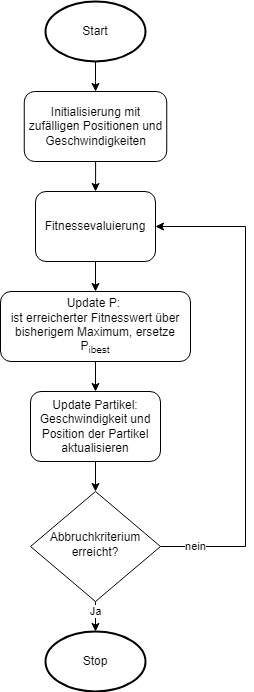
\includegraphics[scale=0.75]{Flow_PSO.png}
  \caption{Flussdiagramm von PSO}
  \label{fig:Figure_PSO}
\end{figure}


\section{Ameisen Algorithmen}
Ameisenalgorithmen sind von der Futtersuche der Ameisen abgeleitet. Jede Ameise scheidet auf ihrem Weg Pheromone aus, welche mit der Zeit verdunsten. 
Folgende Ameisen wählen wahrscheinlicher einen Weg mit größerer Pheromonkonzentration. 
Existieren nun zwei unterschiedlich lange Wege mit gleicher Pheromonkonzentration, entscheiden sich etwa gleich viele Ameisen für beide Wege. 
Da die Ameisen auf dem kürzeren Weg in gleicher Zeit allerdings öfter laufen, steigt hier die Konzentration schneller als auf dem längeren Weg. 
Infolgedessen laufen immer mehr Ameisen den kürzeren Weg und es bildet sich eine Ameisenstraße.\\

Es gibt viele verschiedene Umsetzungen der Ameisenalgorithmen. Der erste Ansatz wurde von Marco Dorigo 1991 vorgestellt\cite{Dorigo1991AntSA} und 1996 nochmal verbessert\cite{484436}.
Sein Ansatz namens \emph{Ant System} lieferte Grundlagen welche er 1997 in einem neuen System namens \emph{Ant Colony System} weiter verbesserte\cite{585892}. In 2000 veröffentlicht Stützle Hoos einen weiteren ACO Algorithmus namens \emph{MAX-MIN Ant System (MMAS)} \cite{STUTZLE2000889} \\
Im Folgenden werden wir erst auf AS eingehen und dann die Unterschiede zu MMAS und ACS erklären.\\
Jede Ameise bewegt sich von Punkt x zu Punkt y mit folgender Wahrscheinlichkeit:\\

\large$p_{xy}^k=\frac{(T_{xy}^a)(n_{xy}^b)}{\Sigma(T_{xy}^a)(n_{xy}^b) }$

\begin{itemize}
  \item $p_{xy}$: Wahrscheinlichkeit des Übergangs von x auf y
  \item $T_x_y$: Menge an Pheromonen auf dem Übergang von x nach y 
  \item a: Gewicht des Einflusses von $T_x_y$
  \item $n_x_y$: Maß wie wünschenswert dieser Übergang ist
  \item b: Gewicht des Einflusses von $n_x_y$
\end{itemize}

$n_{xy}$ wir berechnet durch:\\
$n_{xy}=\frac{1}{d_{xy}}$\\
mit $d_{xy}$ als Abstand zwischen x und y

Nun bewegt sich jeder Agent nach der von ihm berechneten Wahrscheinlichkeit, bis er den Zielzustand erreicht. Außerdem erhält jeder Agent eine taboo Liste der bereits besuchten Zustände, um einen Kreislauf zu verhindern. Dann werden die Pheromone folgendermaßen aktualisiert:\\
$T_{xy}^k=(1-p)T_x_y^k+$\Delta $T_x_y^k$
\begin{itemize}
  \item p: Pheromonverdunstung
  \item k: Nummer der Ameise
  \item $\Delta T_x_y^k$: in diesem Schritt ausgeschüttete Pheromone auf dem Schritt von x nach y
\end{itemize}
$\Delta T_x_y^k$ berechnet sich nun folgendermaßen:

$\Delta T_x_y^k = \left\{
\begin{array}{ll}
\frac{Q}{L_k} & \textrm{wenn Zustand besucht} \\
0 & \, \textrm{sonst} \\
\end{array}
\right. $
\begin{itemize}
    \item Q: Konstanter Wert, wieviel Pheromone ein Agent ausgeschüttete
    \item $L_k$: Länge des Pfades der Ameise
\end{itemize}

Die Wahl der Pheromonverdunstung p hat einen großen Einfluss auf den Erfolg des Algorithmus. Er bestimmt Erkundung und Ausnutzung der Agenten. Ein zu hoher Wert führt zu zuviel Erkundung und das Verlorengehen von Ameisen. Ein zu niedriger Wert schränkt die Erkundung zusehr ein und der optimale Pfad wird unter Umständen nicht gefunden.\\
Das MAX-MIN Ant System(MMAS) wurde eingeführt um die Performance des Systems auf großen Daten zu verbessern. Gegenüber AS gibt es zwei große Unterschiede.  Bei MMAS kann nur der beste Agent die Pheromone verändern. Außerdem gibt es einen maximalen sowie einen minimalen Wert für $T_x_y$. $T_{max} und T_{min}$ werden für ein Problem spezifisch empirisch gewählt\cite{socha2002max}. Allerdings gibt es dafür Richtlinine die bei einer guten Wahl helfen kann\cite*{STUTZLE2000889}.\\ $\Delta T_{xy}$ wird berechnet mit $\Delta T_x_y = \left\{
  \begin{array}{ll}
  \frac{1}{L_{best}} & \textrm{wenn Zustand besucht} \\
  0 & \, \textrm{sonst} \\
  \end{array}
  \right. $
$L_{best}$ kann jetzt entweder der beste bisherige Pfad,der beste Pfad aus der letzten Iteration sein oder eine Kombination der beiden.


Schritte der grundsätzlichen Durchführung von ACO:
\begin{enumerate}
  \item Initialisierung: Die Übergänge zwischen Start und Ziel bekommen einen Wert für n zugewiesen
  \item Jede Einheit bewegt sich einen Schritt übereinstimmend mit der berechneten Wahrscheinlichkeit.  Wiederholen, bis das Ziel erreicht ist
  \item Die Länge der Pfade messen und Pheromonkonzentration aktualisieren
  \item Die Länge aller Pfade mit dem bisherigen besten Pfad vergleichen, den besten Pfad speichern
  \item Wiederholung: Schritt 2-4 wiederholen bis Abbruchkriterium erreicht ist
\end{enumerate}

\begin{figure}
  \centering
  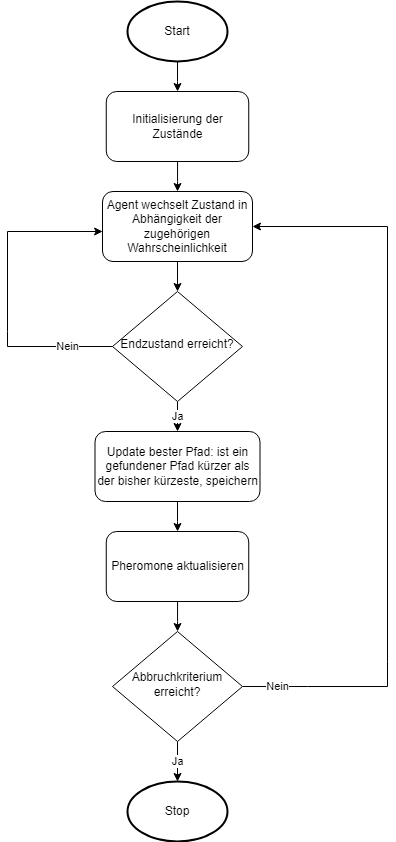
\includegraphics[scale=0.75]{Flow_ACO.png}
  \caption{Flussdiagramm von ACO}
  \label{fig:Figure_ACO}
\end{figure}

\section{Bienen Algorithmen}
Der Bienen Algorithmus ist von der Futtersuche der Bienen abgeleitet. Ein kleiner Teil des Bienenschwarms fungiert als Kundschafter für die Kolonie.
Sie sind konstant zufällig auf der Futtersuche. Finden sie eine Futterquelle analysieren sie deren Effektivität und kehren zum Bienenstock zurück. Die Effektivität hängt von Faktoren wie der Menge, Entfernung und Zuckergehalt ab.\cite{PHAM2006454}
Die Bienen, die eine effektive Futterquelle gefunden haben, führen nun einen sogenannten \emph{waggle dance} auf dem \emph{dance floor} aus \cite{Seeley+1995}. Damit gibt sie die Wegbeschreibung zur Futterquelle weiter.
Unbeschäftigte Arbeiterbienen schauen auf dem dance floor nach Wegbeschreibungen. Umso effektiver die Futterquelle, umso länger der Tanz, daher werden auch mehr Arbeiterbienen diese ausnutzen.\cite{KARABOGA2009108}\\

Im Artificial Bee Colony (ABC) Algorithmus gibt es drei Gruppen an Bienen:
\begin{enumerate}
  \item Kundschafter (Scout) Bienen: Sie fliegen zufällig auf der Futtersuche umher
  \item Betrachtende Bienen: Sie stehen am dance floor und beobachten die Tänze. Sie suchen sich den besten aus und werden nun zu beschäftigten Bienen
  \item Beschäftigte Bienen: Sie fliegen zu der von ihr gewählten Futterquelle. Nachdem sie zurückgekehrt sind kommunizieren sie ihre Informationen auf dem dance floor weiter
\end{enumerate} 

Die Position einer Futterquelle repräsentiert eine mögliche Lösung des Optimierungsproblems, die Effektivität der Futterquelle die damit verbundene Fitness.
Der Algorithmus beginnt mit einem zufälligen Pfad von Start zu Ende. Auf diesem befinden sich Breakpoints, z.B. an Stellen wo ein Hindernis getroffen wird.
Breakpoints sind Stellen an denen sich zwei Geraden treffen. Diese Stellen sind Futterquellen und in ihrer Nähe suchen die jeweiligen Bienen. 
Es gibt immer so viele beschäftigte Bienen wie Futterquellen bzw Pfade. Jede beschäftigte Biene hat einen festen Pfad, den sie versucht zu optimieren\cite{pham2005bees}. 
Die betrachtenden Bienen wählen nun einen Pfad abhängig von folgender Wahrscheinlichkeit:\\
$p_i=\frac{f_i}{\Sigma^N_{n=0}f_n}$
\begin{itemize}
  \item $f_i$: Fitness des Pfades
  \item N: Anzahl aller Pfade
\end{itemize}
Die betrachtenden Bienen versuchen nun den so gewählten Pfad zu verbessern. Kundschafter Bienen suchen zufällig nach neuen Pfaden.\\
Schritte der gründsätzlichen Durchführung des Bienen Algorithmus:
\begin{enumerate}
  \item Initialisierung: Ein initialer Pfad wird gewählt, gerade Linie von Start zu Ende, drehen wenn Hindernis gefunden
  \item Länge des initialen Pfades berechnen
  \item Jedem Breakpoint wird eine beschäftigte Biene zugewiesen, diese versucht ihn zu verbessern
  \item Jeder betrachtenden Bienen wird ein Breakpoint zugewiesen,diese versucht sie zu verbessern
  \item Kundschafter Bienen suchen nach neuen Pfaden
  \item Kann eine Biene einen Pfad verbessern, wird dieser gespeichert
  \item Findet eine Kundschafter Biene einen neuen Pfad wird dieser gespeichert
  \item Wiederholung: Schritt 3-7 wiederholen bis Abbruchkriterium erreicht ist
\end{enumerate}

\begin{figure}
  \centering
  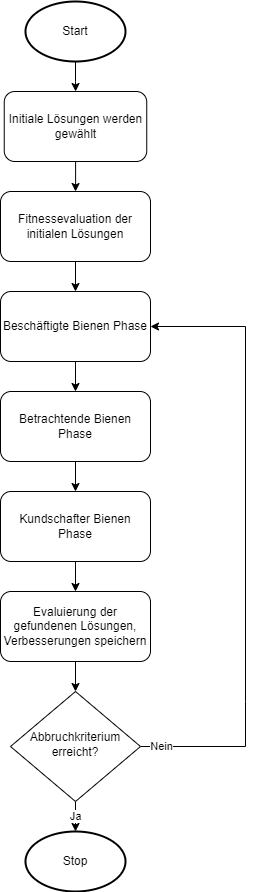
\includegraphics[scale=0.75]{Flow_ABC.png}
  \caption{Flussdiagramm von ABC}
  \label{fig:Figure_ABC}
\end{figure}
